%% knit("Grid_trial_multinomial_fits_v0.Rnw")

\documentclass[12pt]{article}\usepackage[]{graphicx}\usepackage[]{color}
%% maxwidth is the original width if it is less than linewidth
%% otherwise use linewidth (to make sure the graphics do not exceed the margin)
\makeatletter
\def\maxwidth{ %
  \ifdim\Gin@nat@width>\linewidth
    \linewidth
  \else
    \Gin@nat@width
  \fi
}
\makeatother

\definecolor{fgcolor}{rgb}{0.345, 0.345, 0.345}
\newcommand{\hlnum}[1]{\textcolor[rgb]{0.686,0.059,0.569}{#1}}%
\newcommand{\hlstr}[1]{\textcolor[rgb]{0.192,0.494,0.8}{#1}}%
\newcommand{\hlcom}[1]{\textcolor[rgb]{0.678,0.584,0.686}{\textit{#1}}}%
\newcommand{\hlopt}[1]{\textcolor[rgb]{0,0,0}{#1}}%
\newcommand{\hlstd}[1]{\textcolor[rgb]{0.345,0.345,0.345}{#1}}%
\newcommand{\hlkwa}[1]{\textcolor[rgb]{0.161,0.373,0.58}{\textbf{#1}}}%
\newcommand{\hlkwb}[1]{\textcolor[rgb]{0.69,0.353,0.396}{#1}}%
\newcommand{\hlkwc}[1]{\textcolor[rgb]{0.333,0.667,0.333}{#1}}%
\newcommand{\hlkwd}[1]{\textcolor[rgb]{0.737,0.353,0.396}{\textbf{#1}}}%

\usepackage{framed}
\makeatletter
\newenvironment{kframe}{%
 \def\at@end@of@kframe{}%
 \ifinner\ifhmode%
  \def\at@end@of@kframe{\end{minipage}}%
  \begin{minipage}{\columnwidth}%
 \fi\fi%
 \def\FrameCommand##1{\hskip\@totalleftmargin \hskip-\fboxsep
 \colorbox{shadecolor}{##1}\hskip-\fboxsep
     % There is no \\@totalrightmargin, so:
     \hskip-\linewidth \hskip-\@totalleftmargin \hskip\columnwidth}%
 \MakeFramed {\advance\hsize-\width
   \@totalleftmargin\z@ \linewidth\hsize
   \@setminipage}}%
 {\par\unskip\endMakeFramed%
 \at@end@of@kframe}
\makeatother

\definecolor{shadecolor}{rgb}{.97, .97, .97}
\definecolor{messagecolor}{rgb}{0, 0, 0}
\definecolor{warningcolor}{rgb}{1, 0, 1}
\definecolor{errorcolor}{rgb}{1, 0, 0}
\newenvironment{knitrout}{}{} % an empty environment to be redefined in TeX

\usepackage{alltt}
\usepackage{times}
\usepackage{hyperref}
\usepackage{natbib}
\hypersetup{pdfpagemode=UseNone} % don't show bookmarks on initial view
\hypersetup{colorlinks, urlcolor={blue}}

\usepackage{geometry}
\geometry{a4paper, margin=2cm}

\title{Grid trial multinomial fits to the \textit{Nephrops} data}
\author{For discussion only}
\date{\today}
\IfFileExists{upquote.sty}{\usepackage{upquote}}{}
\begin{document}



\maketitle

\section{Data}

\begin{knitrout}\footnotesize
\definecolor{shadecolor}{rgb}{0.969, 0.969, 0.969}\color{fgcolor}\begin{kframe}
\begin{alltt}
\hlkwd{library}\hlstd{(gdata)}

\hlcom{## Nephrops length data}
\hlstd{grid.neph.dat} \hlkwb{<-}
  \hlkwd{read.xls}\hlstd{(}
    \hlstr{"../data/Do_Not_Overwrite_OUR_LASSII_Grid_Trial_FU15_September_2015.xlsx"}\hlstd{,}
    \hlkwc{sheet} \hlstd{=} \hlstr{"Nephrops"}\hlstd{,}
    \hlkwc{stringsAsFactors} \hlstd{=} \hlnum{FALSE}\hlstd{)}

\hlcom{## Remove haul number 4 }
\hlstd{grid.neph.dat} \hlkwb{<-} \hlkwd{subset}\hlstd{(grid.neph.dat, HAUL} \hlopt{!=} \hlnum{4}\hlstd{)}

\hlcom{## Make the "HAUL" variable character}
\hlstd{grid.neph.dat}\hlopt{$}\hlstd{HAUL} \hlkwb{<-} \hlkwd{paste}\hlstd{(}\hlstr{"H"}\hlstd{, grid.neph.dat}\hlopt{$}\hlstd{HAUL,} \hlkwc{sep} \hlstd{=}\hlstr{""}\hlstd{)}

\hlcom{## make some factor variables used in the analyses}
\hlstd{grid.neph.dat}\hlopt{$}\hlstd{fHAUL} \hlkwb{<-} \hlkwd{factor}\hlstd{(grid.neph.dat}\hlopt{$}\hlstd{HAUL,} \hlkwc{levels} \hlstd{=} \hlkwd{unique}\hlstd{(grid.neph.dat}\hlopt{$}\hlstd{HAUL))}
\hlstd{grid.neph.dat}\hlopt{$}\hlstd{COMPARTMENT} \hlkwb{<-} \hlkwd{factor}\hlstd{(grid.neph.dat}\hlopt{$}\hlstd{COMPARTMENT)}

\hlcom{## NOT REMOVING HERE}
\hlcom{## remove observations above 99th and below 1th length percentile}
\hlcom{## these can be highly influential on the fits}
\hlcom{##grid.neph.dat <- subset(grid.neph.dat, Carapace.length < quantile(Carapace.length, 0.99) &}
\hlcom{##                   Carapace.length > quantile(Carapace.length, 0.01)}
\hlcom{##                   )}

\hlcom{## change a few names }
\hlkwd{names}\hlstd{(grid.neph.dat)[}\hlkwd{names}\hlstd{(grid.neph.dat)} \hlopt{==} \hlstr{"CARAPACE.LENGTH..mm."}\hlstd{]} \hlkwb{<-} \hlstr{"Carapace.length"}
\hlkwd{names}\hlstd{(grid.neph.dat)[}\hlkwd{names}\hlstd{(grid.neph.dat)} \hlopt{==} \hlstr{"BULK.CATCH...kg."}\hlstd{]} \hlkwb{<-} \hlstr{"Bulk.weight"}

\hlcom{## Show the first 2 rows}
\hlkwd{head}\hlstd{(grid.neph.dat,} \hlnum{2}\hlstd{)}
\end{alltt}
\begin{verbatim}
##   HAUL COMPARTMENT Carapace.length COUNT RAISED.COUNT Bulk.weight
## 1   H1          SG              13     2           NA         132
## 2   H1          SG              15     3           NA         132
##   BULK.CATCH.SUBSAMPLE.WEIGHT..kg. BULK.CATCH.SUBSAMPLE.RATIO
## 1                              132                          1
## 2                              132                          1
##   NEPHROPS.WEIGHT.IN.SUBSAMPLE..kg.
## 1                              89.6
## 2                              89.6
##   SUBSAMPLE.OF.NEPHROPS.FOR.MEASUREMENT..kg. NEPHROPS.SUBSAMPLE.RATIO
## 1                                        5.2                 17.23077
## 2                                        5.2                 17.23077
##   OVERALL.RAISING.FACTOR OVERALL.SUBS.RATIO fHAUL
## 1               17.23077         0.05803571    H1
## 2               17.23077         0.05803571    H1
\end{verbatim}
\begin{alltt}
\hlcom{## Bring in rotation data (used further down)}
\hlstd{rotation.dat} \hlkwb{<-}
  \hlkwd{read.xls}\hlstd{(}
    \hlstr{"../data/Do_Not_Overwrite_OUR_LASSII_Grid_Trial_FU15_September_2015.xlsx"}\hlstd{,}
    \hlkwc{sheet} \hlstd{=} \hlstr{"Rotations"}\hlstd{,}
    \hlkwc{stringsAsFactors} \hlstd{=} \hlnum{FALSE}\hlstd{,} \hlkwc{nrows} \hlstd{=} \hlnum{13}\hlstd{)}

\hlcom{## need to create a rotation variable}
\hlcom{## use short codes for rotation names}
\hlcom{## starboard outside}
\hlstd{rotation.dat}\hlopt{$}\hlstd{SO} \hlkwb{<-} \hlnum{NA}
\hlstd{rotation.dat}\hlopt{$}\hlstd{SO[rotation.dat}\hlopt{$}\hlstd{Starboard.Outside} \hlopt{==} \hlstr{"Nephrops sorting grid 1"}\hlstd{]} \hlkwb{<-} \hlstr{"NSG1"}
\hlstd{rotation.dat}\hlopt{$}\hlstd{SO[rotation.dat}\hlopt{$}\hlstd{Starboard.Outside} \hlopt{==} \hlstr{"Nephrops sorting grid 2"}\hlstd{]} \hlkwb{<-} \hlstr{"NSG2"}
\hlstd{rotation.dat}\hlopt{$}\hlstd{SO[rotation.dat}\hlopt{$}\hlstd{Starboard.Outside} \hlopt{==} \hlstr{"Swedish grid"}\hlstd{]} \hlkwb{<-} \hlstr{"SG"}
\hlstd{rotation.dat}\hlopt{$}\hlstd{SO[rotation.dat}\hlopt{$}\hlstd{Starboard.Outside} \hlopt{==} \hlstr{"Control 70mm"}\hlstd{]} \hlkwb{<-} \hlstr{"CTRL"}

\hlcom{## starboard inside}
\hlstd{rotation.dat}\hlopt{$}\hlstd{SI} \hlkwb{<-} \hlnum{NA}
\hlstd{rotation.dat}\hlopt{$}\hlstd{SI[rotation.dat}\hlopt{$}\hlstd{Starboard.Inside} \hlopt{==} \hlstr{"Nephrops sorting grid 1"}\hlstd{]} \hlkwb{<-} \hlstr{"NSG1"}
\hlstd{rotation.dat}\hlopt{$}\hlstd{SI[rotation.dat}\hlopt{$}\hlstd{Starboard.Inside} \hlopt{==} \hlstr{"Nephrops sorting grid 2"}\hlstd{]} \hlkwb{<-} \hlstr{"NSG2"}
\hlstd{rotation.dat}\hlopt{$}\hlstd{SI[rotation.dat}\hlopt{$}\hlstd{Starboard.Inside} \hlopt{==} \hlstr{"Swedish grid"}\hlstd{]} \hlkwb{<-} \hlstr{"SG"}
\hlstd{rotation.dat}\hlopt{$}\hlstd{SI[rotation.dat}\hlopt{$}\hlstd{Starboard.Inside} \hlopt{==} \hlstr{"Control 70mm"}\hlstd{]} \hlkwb{<-} \hlstr{"CTRL"}

\hlcom{## Port outside}
\hlstd{rotation.dat}\hlopt{$}\hlstd{PO} \hlkwb{<-} \hlnum{NA}
\hlstd{rotation.dat}\hlopt{$}\hlstd{PO[rotation.dat}\hlopt{$}\hlstd{Port.Outside} \hlopt{==} \hlstr{"Nephrops sorting grid 1"}\hlstd{]} \hlkwb{<-} \hlstr{"NSG1"}
\hlstd{rotation.dat}\hlopt{$}\hlstd{PO[rotation.dat}\hlopt{$}\hlstd{Port.Outside} \hlopt{==} \hlstr{"Nephrops sorting grid 2"}\hlstd{]} \hlkwb{<-} \hlstr{"NSG2"}
\hlstd{rotation.dat}\hlopt{$}\hlstd{PO[rotation.dat}\hlopt{$}\hlstd{Port.Outside} \hlopt{==} \hlstr{"Swedish grid"}\hlstd{]} \hlkwb{<-} \hlstr{"SG"}
\hlstd{rotation.dat}\hlopt{$}\hlstd{PO[rotation.dat}\hlopt{$}\hlstd{Port.Outside} \hlopt{==} \hlstr{"Control 70mm"}\hlstd{]} \hlkwb{<-} \hlstr{"CTRL"}

\hlcom{## Port inside}
\hlstd{rotation.dat}\hlopt{$}\hlstd{PI} \hlkwb{<-} \hlnum{NA}
\hlstd{rotation.dat}\hlopt{$}\hlstd{PI[rotation.dat}\hlopt{$}\hlstd{Port.Inside} \hlopt{==} \hlstr{"Nephrops sorting grid 1"}\hlstd{]} \hlkwb{<-} \hlstr{"NSG1"}
\hlstd{rotation.dat}\hlopt{$}\hlstd{PI[rotation.dat}\hlopt{$}\hlstd{Port.Inside} \hlopt{==} \hlstr{"Nephrops sorting grid 2"}\hlstd{]} \hlkwb{<-} \hlstr{"NSG2"}
\hlstd{rotation.dat}\hlopt{$}\hlstd{PI[rotation.dat}\hlopt{$}\hlstd{Port.Inside} \hlopt{==} \hlstr{"Swedish grid"}\hlstd{]} \hlkwb{<-} \hlstr{"SG"}
\hlstd{rotation.dat}\hlopt{$}\hlstd{PI[rotation.dat}\hlopt{$}\hlstd{Port.Inside} \hlopt{==} \hlstr{"Control 70mm"}\hlstd{]} \hlkwb{<-} \hlstr{"CTRL"}

\hlcom{## get a unique net configuration variable}
\hlstd{rotation.dat}\hlopt{$}\hlstd{netconfig} \hlkwb{<-} \hlkwd{with}\hlstd{(rotation.dat,} \hlkwd{paste}\hlstd{(SO, SI, PO, PI,} \hlkwc{sep} \hlstd{=} \hlstr{":"}\hlstd{))}

\hlstd{rotation.dat}\hlopt{$}\hlstd{HAUL} \hlkwb{<-} \hlkwd{paste}\hlstd{(}\hlstr{"H"}\hlstd{, rotation.dat}\hlopt{$}\hlstd{Haul..,} \hlkwc{sep} \hlstd{=} \hlstr{""}\hlstd{)}
\hlstd{rotation.dat}\hlopt{$}\hlstd{fHAUL} \hlkwb{<-} \hlkwd{factor}\hlstd{(rotation.dat}\hlopt{$}\hlstd{HAUL,} \hlkwc{levels} \hlstd{=} \hlkwd{unique}\hlstd{(rotation.dat}\hlopt{$}\hlstd{HAUL))}
\end{alltt}
\end{kframe}
\end{knitrout}

Data pre-processing to format needed for model fits

\begin{knitrout}\footnotesize
\definecolor{shadecolor}{rgb}{0.969, 0.969, 0.969}\color{fgcolor}\begin{kframe}
\begin{alltt}
\hlcom{## get count per length bin per haul by mesh size}
\hlcom{## using the reshape package (makes it easier to process data)}
\hlkwd{library}\hlstd{(reshape)}

\hlcom{## variables to keep }
\hlstd{vars2keep} \hlkwb{<-} \hlkwd{c}\hlstd{(}\hlstr{"COMPARTMENT"}\hlstd{,} \hlstr{"Carapace.length"}\hlstd{,} \hlstr{"fHAUL"}\hlstd{,} \hlstr{"COUNT"}\hlstd{)}

\hlcom{## melt the data frame}
\hlstd{grid.neph.melt} \hlkwb{<-} \hlkwd{melt}\hlstd{(grid.neph.dat[, vars2keep],}
                  \hlkwc{id} \hlstd{=} \hlkwd{c}\hlstd{(}\hlstr{"COMPARTMENT"}\hlstd{,} \hlstr{"Carapace.length"}\hlstd{,} \hlstr{"fHAUL"}\hlstd{))}

\hlcom{## re-form the dataframe in required format }
\hlstd{grid.neph.cast} \hlkwb{<-} \hlkwd{cast}\hlstd{(grid.neph.melt, Carapace.length} \hlopt{+} \hlstd{fHAUL}  \hlopt{~} \hlstd{COMPARTMENT}  \hlopt{+} \hlstd{variable)}
\hlstd{grid.neph.cast} \hlkwb{<-} \hlstd{grid.neph.cast[}\hlkwd{order}\hlstd{(grid.neph.cast}\hlopt{$}\hlstd{fHAUL, grid.neph.cast}\hlopt{$}\hlstd{Carapace.length), ]}
\hlstd{grid.neph.cast[}\hlkwd{is.na}\hlstd{(grid.neph.cast)]} \hlkwb{<-} \hlnum{0}

\hlcom{## merge in the net position}
\hlstd{grid.neph.cast} \hlkwb{<-} \hlkwd{merge}\hlstd{(grid.neph.cast, rotation.dat[,} \hlkwd{c}\hlstd{(}\hlstr{"fHAUL"}\hlstd{,} \hlstr{"netconfig"}\hlstd{)])}

\hlcom{## merge in the bulk weights}
\hlstd{bulk.weight.melt} \hlkwb{<-} \hlkwd{melt}\hlstd{(}\hlkwd{unique}\hlstd{(grid.neph.dat[ ,} \hlkwd{c}\hlstd{(}\hlstr{"fHAUL"}\hlstd{,} \hlstr{"COMPARTMENT"}\hlstd{,} \hlstr{"Bulk.weight"}\hlstd{)]),}
                         \hlkwc{id} \hlstd{=} \hlkwd{c}\hlstd{(}\hlstr{"COMPARTMENT"}\hlstd{,} \hlstr{"fHAUL"}\hlstd{))}

\hlstd{bulk.weight.cast} \hlkwb{<-} \hlkwd{cast}\hlstd{(bulk.weight.melt, fHAUL}  \hlopt{~} \hlstd{COMPARTMENT}  \hlopt{+} \hlstd{variable)}

\hlstd{grid.neph.cast} \hlkwb{<-} \hlkwd{merge}\hlstd{(grid.neph.cast, bulk.weight.cast)}

\hlcom{## show the first few rows}
\hlkwd{head}\hlstd{(grid.neph.cast,} \hlnum{2}\hlstd{)}
\end{alltt}
\begin{verbatim}
##   fHAUL Carapace.length CTRL_COUNT NSG1_COUNT NSG2_COUNT SG_COUNT
## 1    H1              13          0          0          0        2
## 2    H1              15          0          1          0        3
##           netconfig CTRL_Bulk.weight NSG1_Bulk.weight NSG2_Bulk.weight
## 1 NSG1:SG:CTRL:NSG2           375.75            467.5            294.7
## 2 NSG1:SG:CTRL:NSG2           375.75            467.5            294.7
##   SG_Bulk.weight
## 1            132
## 2            132
\end{verbatim}
\begin{alltt}
\hlcom{## format the subsampling ratio similarly}

\hlcom{## double-check that there are unique raising factors per haul}
\hlstd{rf.count} \hlkwb{<-} \hlkwd{with}\hlstd{(grid.neph.dat,} \hlkwd{table}\hlstd{(fHAUL, OVERALL.SUBS.RATIO, COMPARTMENT))}
\hlkwd{apply}\hlstd{(rf.count,} \hlnum{1}\hlstd{,} \hlkwc{FUN} \hlstd{=} \hlkwa{function}\hlstd{(}\hlkwc{x}\hlstd{)\{}\hlkwd{sum}\hlstd{(x}\hlopt{>}\hlnum{0}\hlstd{)\})} \hlcom{## yes}
\end{alltt}
\begin{verbatim}
##  H1  H2  H3  H5  H6  H7  H8  H9 H10 H11 H12 H13 
##   4   4   4   4   4   4   4   4   4   4   4   4
\end{verbatim}
\begin{alltt}
\hlcom{## convert to sub-sampling ratio as in Celtic Warrior}
\hlkwd{names}\hlstd{(grid.neph.dat)[}\hlkwd{names}\hlstd{(grid.neph.dat)} \hlopt{==} \hlstr{"OVERALL.SUBS.RATIO"}\hlstd{]} \hlkwb{<-} \hlstr{"SUBSRATIO"}
\hlstd{vars2keep} \hlkwb{<-} \hlkwd{c}\hlstd{(}\hlstr{"COMPARTMENT"}\hlstd{,} \hlstr{"fHAUL"}\hlstd{,} \hlstr{"SUBSRATIO"}\hlstd{)}
\hlstd{subs.melt} \hlkwb{<-} \hlkwd{melt}\hlstd{(}\hlkwd{unique}\hlstd{(grid.neph.dat[, vars2keep]),} \hlkwc{id} \hlstd{=} \hlkwd{c}\hlstd{(}\hlstr{"COMPARTMENT"}\hlstd{,} \hlstr{"fHAUL"}\hlstd{))}
\hlstd{subs.cast} \hlkwb{<-} \hlkwd{cast}\hlstd{(subs.melt, fHAUL}  \hlopt{~} \hlstd{COMPARTMENT} \hlopt{+} \hlstd{variable)}

\hlcom{## merge counts and subsampling ratio back together }
\hlstd{grid.neph.cast} \hlkwb{<-} \hlkwd{merge}\hlstd{(grid.neph.cast, subs.cast,} \hlkwc{by} \hlstd{=} \hlstr{"fHAUL"}\hlstd{,} \hlkwc{all.x} \hlstd{=} \hlnum{TRUE}\hlstd{)}

\hlcom{## show first few lines}
\hlcom{## Note that this is how the data look just prior to analysis}
\hlkwd{head}\hlstd{(grid.neph.cast,} \hlnum{2}\hlstd{)}
\end{alltt}
\begin{verbatim}
##   fHAUL Carapace.length CTRL_COUNT NSG1_COUNT NSG2_COUNT SG_COUNT
## 1    H1              13          0          0          0        2
## 2    H1              15          0          1          0        3
##           netconfig CTRL_Bulk.weight NSG1_Bulk.weight NSG2_Bulk.weight
## 1 NSG1:SG:CTRL:NSG2           375.75            467.5            294.7
## 2 NSG1:SG:CTRL:NSG2           375.75            467.5            294.7
##   SG_Bulk.weight CTRL_SUBSRATIO NSG1_SUBSRATIO NSG2_SUBSRATIO SG_SUBSRATIO
## 1            132     0.05051344      0.0614082       0.140078   0.05803571
## 2            132     0.05051344      0.0614082       0.140078   0.05803571
\end{verbatim}
\end{kframe}
\end{knitrout}

Extract the data in exact format for a multinomial fit.  

\begin{knitrout}\footnotesize
\definecolor{shadecolor}{rgb}{0.969, 0.969, 0.969}\color{fgcolor}\begin{kframe}
\begin{alltt}
\hlcom{## Extract the matrix of counts}
\hlstd{count.vars} \hlkwb{<-} \hlkwd{c}\hlstd{(}\hlstr{"CTRL_COUNT"}\hlstd{,} \hlstr{"NSG1_COUNT"}\hlstd{,} \hlstr{"NSG2_COUNT"}\hlstd{,} \hlstr{"SG_COUNT"}\hlstd{)}

\hlstd{neph.count.mat} \hlkwb{<-} \hlkwd{as.matrix}\hlstd{(grid.neph.cast[, count.vars])}

\hlcom{## Extract the matrix of subsampling ratios}
\hlstd{subsratio.vars} \hlkwb{<-} \hlkwd{c}\hlstd{(}\hlstr{"CTRL_SUBSRATIO"}\hlstd{,} \hlstr{"NSG1_SUBSRATIO"}\hlstd{,} \hlstr{"NSG2_SUBSRATIO"}\hlstd{,} \hlstr{"SG_SUBSRATIO"}\hlstd{)}

\hlstd{subsratio.mat} \hlkwb{<-} \hlkwd{as.matrix}\hlstd{(grid.neph.cast[, subsratio.vars])}

\hlcom{## Create the offset}
\hlstd{offset.mat} \hlkwb{<-} \hlkwd{log}\hlstd{(subsratio.mat} \hlopt{/} \hlstd{subsratio.mat[,}\hlnum{1}\hlstd{])}
\end{alltt}
\end{kframe}
\end{knitrout}

Plot the data 
\begin{knitrout}\footnotesize
\definecolor{shadecolor}{rgb}{0.969, 0.969, 0.969}\color{fgcolor}\begin{kframe}
\begin{alltt}
\hlkwd{library}\hlstd{(ggplot2)}

\hlcom{## N.B. to plot the proportions correctly, use the raised counts}
\hlcom{## raised count per compartment and haul and carapace length}
\hlstd{raised.count.compartment} \hlkwb{<-} \hlstd{neph.count.mat} \hlopt{/} \hlstd{subsratio.mat}

\hlcom{## Get the proportions}
\hlstd{prop.compartment} \hlkwb{<-} \hlkwd{prop.table}\hlstd{(raised.count.compartment,} \hlkwc{margin} \hlstd{=} \hlnum{1}\hlstd{)}

\hlstd{m} \hlkwb{<-} \hlkwd{dim}\hlstd{(prop.compartment)[}\hlnum{1}\hlstd{]}

\hlcom{## make a dataframe of the proportions for ggplot}
\hlstd{prop.compartment.df} \hlkwb{<-} \hlkwd{data.frame}\hlstd{(}
                         \hlkwc{proportion} \hlstd{=} \hlkwd{c}\hlstd{(prop.compartment),}
                         \hlkwc{count} \hlstd{=} \hlkwd{c}\hlstd{(raised.count.compartment),}
                         \hlkwc{Carapace.length} \hlstd{=} \hlkwd{rep}\hlstd{(grid.neph.cast}\hlopt{$}\hlstd{Carapace.length,} \hlkwc{times} \hlstd{=} \hlnum{4}\hlstd{),}
                         \hlkwc{COMPARTMENT} \hlstd{=} \hlkwd{rep}\hlstd{(}\hlkwd{c}\hlstd{(}\hlstr{"Control"}\hlstd{,} \hlstr{"Nephrops sorting grid 1"}\hlstd{,}
                           \hlstr{"Nephrops sorting grid 2"}\hlstd{,} \hlstr{"Swedish grid"}\hlstd{),} \hlkwc{each} \hlstd{= m)}
                         \hlstd{)}

\hlkwd{theme_set}\hlstd{(}\hlkwd{theme_bw}\hlstd{())}

\hlstd{p} \hlkwb{<-} \hlkwd{ggplot}\hlstd{(prop.compartment.df,} \hlkwd{aes}\hlstd{(}\hlkwc{x} \hlstd{= Carapace.length,} \hlkwc{y} \hlstd{= proportion))} \hlopt{+}
  \hlkwd{geom_point}\hlstd{(}\hlkwc{colour} \hlstd{=} \hlstr{"#F8766D"}\hlstd{,} \hlkwc{alpha} \hlstd{=} \hlnum{0.2}\hlstd{,} \hlkwd{aes}\hlstd{(}\hlkwc{size} \hlstd{=} \hlnum{2}\hlopt{*}\hlkwd{log}\hlstd{(count)))} \hlopt{+}
\hlkwd{facet_wrap}\hlstd{(}\hlopt{~} \hlstd{COMPARTMENT)} \hlopt{+} \hlkwd{ylab}\hlstd{(}\hlstr{"Proportion of Nephrops per compartment"}\hlstd{)} \hlopt{+}
  \hlkwd{theme}\hlstd{(}\hlkwc{legend.position} \hlstd{=} \hlstr{"bottom"}\hlstd{)}

\hlstd{p}
\end{alltt}
\end{kframe}\begin{figure}
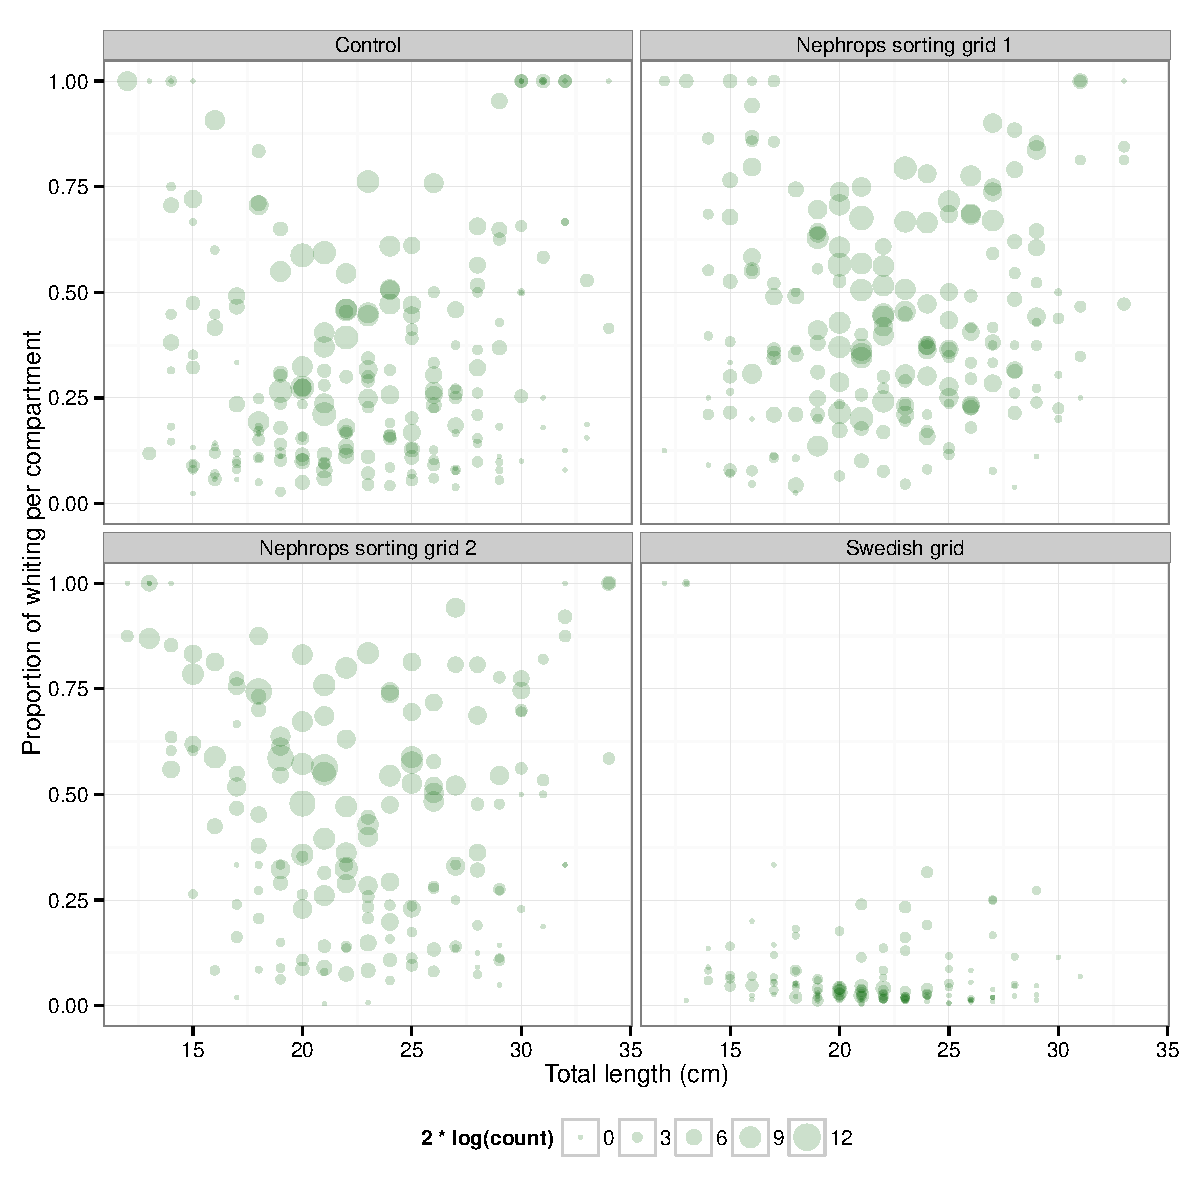
\includegraphics[width=\maxwidth]{figure/unnamed-chunk-5-1} \caption[Proportion of Nephrops catch retained per haul]{Proportion of Nephrops catch retained per haul. Each point represents the proportion of raised Nephrops catch per haul and length class retained in a given cod-end (Control: CTRL, Nephrops Sorting grid 1: NSG1, Nephrops Sorting grid 2: NSG2, or the Swedish Grid). The size of the point is proportional to the log of the count.}\label{fig:unnamed-chunk-5}
\end{figure}


\end{knitrout}

\section{Model}
The first model we can use is a multinomial for the proportion retained in the four compartments. 

\begin{knitrout}\footnotesize
\definecolor{shadecolor}{rgb}{0.969, 0.969, 0.969}\color{fgcolor}\begin{kframe}
\begin{alltt}
\hlkwd{library}\hlstd{(nnet)}

\hlcom{## First fit is constant proportions}
\hlcom{## not accounting for length}

\hlstd{mnom0} \hlkwb{<-} \hlkwd{multinom}\hlstd{(neph.count.mat} \hlopt{~} \hlnum{1} \hlopt{+} \hlkwd{offset}\hlstd{(offset.mat))}
\end{alltt}
\begin{verbatim}
## # weights:  24 (3 variable)
## initial  value 28451.789893 
## final  value 28311.405094 
## converged
\end{verbatim}
\begin{alltt}
\hlcom{## second fit include net configuration/rotations}
\hlstd{mnom0.1} \hlkwb{<-} \hlkwd{multinom}\hlstd{(neph.count.mat} \hlopt{~} \hlstd{netconfig} \hlopt{+}
                    \hlkwd{offset}\hlstd{(offset.mat),} \hlkwc{data} \hlstd{= grid.neph.cast)}
\end{alltt}
\begin{verbatim}
## # weights:  36 (12 variable)
## initial  value 28451.789893 
## iter  10 value 27887.473369
## final  value 27749.753260 
## converged
\end{verbatim}
\begin{alltt}
\hlcom{## include carapace length polynomials of different complexity}
\hlstd{mnom1} \hlkwb{<-} \hlkwd{update}\hlstd{(mnom0.1, .} \hlopt{~} \hlstd{.} \hlopt{+} \hlkwd{poly}\hlstd{(Carapace.length,} \hlnum{1}\hlstd{),}
                \hlkwc{data} \hlstd{= grid.neph.cast)}
\end{alltt}
\begin{verbatim}
## # weights:  40 (15 variable)
## initial  value 28451.789893 
## iter  10 value 27869.288971
## final  value 27696.063407 
## converged
\end{verbatim}
\begin{alltt}
\hlstd{mnom2} \hlkwb{<-} \hlkwd{update}\hlstd{(mnom0.1, .} \hlopt{~} \hlstd{.} \hlopt{+} \hlkwd{poly}\hlstd{(Carapace.length,} \hlnum{2}\hlstd{),}
                \hlkwc{data} \hlstd{= grid.neph.cast)}
\end{alltt}
\begin{verbatim}
## # weights:  44 (18 variable)
## initial  value 28451.789893 
## iter  10 value 27861.252166
## iter  20 value 27691.533797
## iter  20 value 27691.533734
## iter  20 value 27691.533734
## final  value 27691.533734 
## converged
\end{verbatim}
\begin{alltt}
\hlstd{mnom3} \hlkwb{<-} \hlkwd{update}\hlstd{(mnom0.1, .} \hlopt{~} \hlstd{.} \hlopt{+} \hlkwd{poly}\hlstd{(Carapace.length,} \hlnum{3}\hlstd{),} \hlkwc{data} \hlstd{= grid.neph.cast)}
\end{alltt}
\begin{verbatim}
## # weights:  48 (21 variable)
## initial  value 28451.789893 
## iter  10 value 27855.790341
## iter  20 value 27690.817351
## final  value 27690.682490 
## converged
\end{verbatim}
\begin{alltt}
\hlkwd{AIC}\hlstd{(mnom0, mnom0.1, mnom1, mnom2, mnom3)}
\end{alltt}
\begin{verbatim}
##         df      AIC
## mnom0    3 56628.81
## mnom0.1 12 55523.51
## mnom1   15 55422.13
## mnom2   18 55419.07
## mnom3   21 55423.36
\end{verbatim}
\begin{alltt}
\hlcom{## looks like a quadratic carapace length effect fits best}
\end{alltt}
\end{kframe}
\end{knitrout}


Get predictions for the fitted model (note that this is run in a cleaner fashion in the ADMB fit below).

\begin{knitrout}\footnotesize
\definecolor{shadecolor}{rgb}{0.969, 0.969, 0.969}\color{fgcolor}\begin{kframe}
\begin{alltt}
\hlcom{## get predictions manually}
\hlcom{## CIs not defined in multinomial context but let's try}

\hlstd{best.model} \hlkwb{<-} \hlstd{mnom2}

\hlcom{## fit coefficients}
\hlstd{beta.mu} \hlkwb{<-} \hlkwd{c}\hlstd{(}\hlkwd{t}\hlstd{(}\hlkwd{coef}\hlstd{(best.model)))}

\hlcom{## fit coefficient variance covariance matrix}
\hlstd{Sigma} \hlkwb{<-} \hlkwd{vcov}\hlstd{(best.model)}

\hlcom{## number of lengths to predict for}
\hlstd{nlength} \hlkwb{<-} \hlnum{50}

\hlstd{pred.length} \hlkwb{<-} \hlkwd{seq}\hlstd{(}\hlkwd{min}\hlstd{(grid.neph.cast}\hlopt{$}\hlstd{Carapace.length),}
                   \hlkwd{max}\hlstd{(grid.neph.cast}\hlopt{$}\hlstd{Carapace.length),} \hlkwc{length} \hlstd{= nlength)}

\hlcom{## get the polynomial of lengths}
\hlstd{polyfun} \hlkwb{<-} \hlkwd{poly}\hlstd{(grid.neph.cast}\hlopt{$}\hlstd{Carapace.length,} \hlnum{2}\hlstd{)}

\hlcom{## model matrix}
\hlstd{Xpred} \hlkwb{<-} \hlkwd{cbind}\hlstd{(}\hlnum{1}\hlstd{,} \hlnum{1}\hlopt{/}\hlnum{3}\hlstd{,} \hlnum{1}\hlopt{/}\hlnum{3}\hlstd{,} \hlnum{1}\hlopt{/}\hlnum{3}\hlstd{,} \hlkwd{predict}\hlstd{(polyfun, pred.length))}

\hlcom{## number of times to resample predictions to get CIs}
\hlstd{nresamp} \hlkwb{<-} \hlnum{1e3}
\hlstd{pred.array} \hlkwb{<-} \hlkwd{array}\hlstd{(}\hlnum{NA}\hlstd{,} \hlkwc{dim} \hlstd{=} \hlkwd{c}\hlstd{(nlength,} \hlnum{4}\hlstd{, nresamp))}

\hlcom{## package to draw from multivariate normal }
\hlkwd{library}\hlstd{(mvtnorm)}

\hlkwa{for}\hlstd{(i} \hlkwa{in} \hlnum{1}\hlopt{:}\hlstd{nresamp)\{}
  \hlcom{##print(i)}
  \hlstd{beta0} \hlkwb{<-} \hlkwd{matrix}\hlstd{(}\hlkwd{rmvnorm}\hlstd{(}\hlnum{1}\hlstd{,} \hlkwc{mean} \hlstd{= beta.mu,} \hlkwc{sigma} \hlstd{= Sigma),}
                  \hlkwc{nrow} \hlstd{=} \hlnum{3}\hlstd{,} \hlkwc{byrow} \hlstd{=} \hlnum{TRUE}\hlstd{)}
  \hlstd{beta} \hlkwb{<-} \hlkwd{cbind}\hlstd{(}\hlnum{0}\hlstd{,} \hlkwd{t}\hlstd{(beta0))}
  \hlstd{eta} \hlkwb{<-} \hlstd{Xpred} \hlopt \hlstd{beta}
  \hlstd{pred.p} \hlkwb{<-} \hlkwd{exp}\hlstd{(eta)} \hlopt{/} \hlkwd{rowSums}\hlstd{(}\hlkwd{exp}\hlstd{(eta))}
  \hlstd{pred.array[ , , i]} \hlkwb{<-} \hlstd{pred.p}
  \hlkwd{rm}\hlstd{(pred.p)}
\hlstd{\}}

\hlcom{## mean across samples}
\hlstd{pred.mu} \hlkwb{<-} \hlkwd{apply}\hlstd{(pred.array,} \hlkwd{c}\hlstd{(}\hlnum{1}\hlstd{,} \hlnum{2}\hlstd{), mean)}

\hlcom{## upper across samples}
\hlstd{pred.upper} \hlkwb{<-} \hlkwd{apply}\hlstd{(pred.array,} \hlkwd{c}\hlstd{(}\hlnum{1}\hlstd{,} \hlnum{2}\hlstd{), quantile,} \hlkwc{p} \hlstd{=} \hlnum{0.975}\hlstd{)}

\hlcom{## lower across samples}
\hlstd{pred.lower} \hlkwb{<-} \hlkwd{apply}\hlstd{(pred.array,} \hlkwd{c}\hlstd{(}\hlnum{1}\hlstd{,} \hlnum{2}\hlstd{), quantile,} \hlkwc{p} \hlstd{=} \hlnum{0.025}\hlstd{)}

\hlcom{## bring all together in a data frame for ggplot}
\hlstd{m} \hlkwb{<-} \hlkwd{dim}\hlstd{(pred.mu)[}\hlnum{1}\hlstd{]}

\hlstd{pred.ci.df} \hlkwb{<-} \hlkwd{data.frame}\hlstd{(}
                \hlkwc{COMPARTMENT} \hlstd{=} \hlkwd{rep}\hlstd{(}\hlkwd{c}\hlstd{(}\hlstr{"Control"}\hlstd{,} \hlstr{"Nephrops sorting grid 1"}\hlstd{,}
                  \hlstr{"Nephrops sorting grid 2"}\hlstd{,} \hlstr{"Swedish grid"}\hlstd{),} \hlkwc{each} \hlstd{= m),}
                \hlkwc{Carapace.length} \hlstd{=} \hlkwd{rep}\hlstd{(pred.length,} \hlkwc{times} \hlstd{=} \hlnum{4}\hlstd{),}
                \hlkwc{proportion} \hlstd{=} \hlkwd{c}\hlstd{(pred.mu),}
                \hlkwc{lower} \hlstd{=} \hlkwd{c}\hlstd{(pred.lower),}
                \hlkwc{upper} \hlstd{=} \hlkwd{c}\hlstd{(pred.upper))}
\end{alltt}
\end{kframe}
\end{knitrout}

Finally overlay the fit on the sample proportions

\begin{knitrout}\footnotesize
\definecolor{shadecolor}{rgb}{0.969, 0.969, 0.969}\color{fgcolor}\begin{kframe}
\begin{alltt}
\hlstd{p} \hlopt{+} \hlkwd{geom_ribbon}\hlstd{(}\hlkwc{data} \hlstd{= pred.ci.df,} \hlkwd{aes}\hlstd{(}\hlkwc{ymin} \hlstd{= lower,} \hlkwc{ymax} \hlstd{= upper),}
                \hlkwc{alpha} \hlstd{=} \hlnum{0.3}\hlstd{,} \hlkwc{fill} \hlstd{=} \hlstr{"blue"}\hlstd{)} \hlopt{+}
  \hlkwd{geom_line}\hlstd{(}\hlkwc{data} \hlstd{= pred.ci.df,} \hlkwd{aes}\hlstd{(}\hlkwc{x} \hlstd{= Carapace.length,} \hlkwc{y} \hlstd{= proportion),}
            \hlkwc{col} \hlstd{=} \hlstr{"navy"}\hlstd{,} \hlkwc{size} \hlstd{=} \hlnum{0.5}\hlstd{)} \hlopt{+}
  \hlkwd{geom_hline}\hlstd{(}\hlkwd{aes}\hlstd{(}\hlkwc{yintercept} \hlstd{=} \hlnum{0.25}\hlstd{),} \hlkwc{linetype} \hlstd{=} \hlstr{"dashed"}\hlstd{)}
\end{alltt}
\end{kframe}\begin{figure}
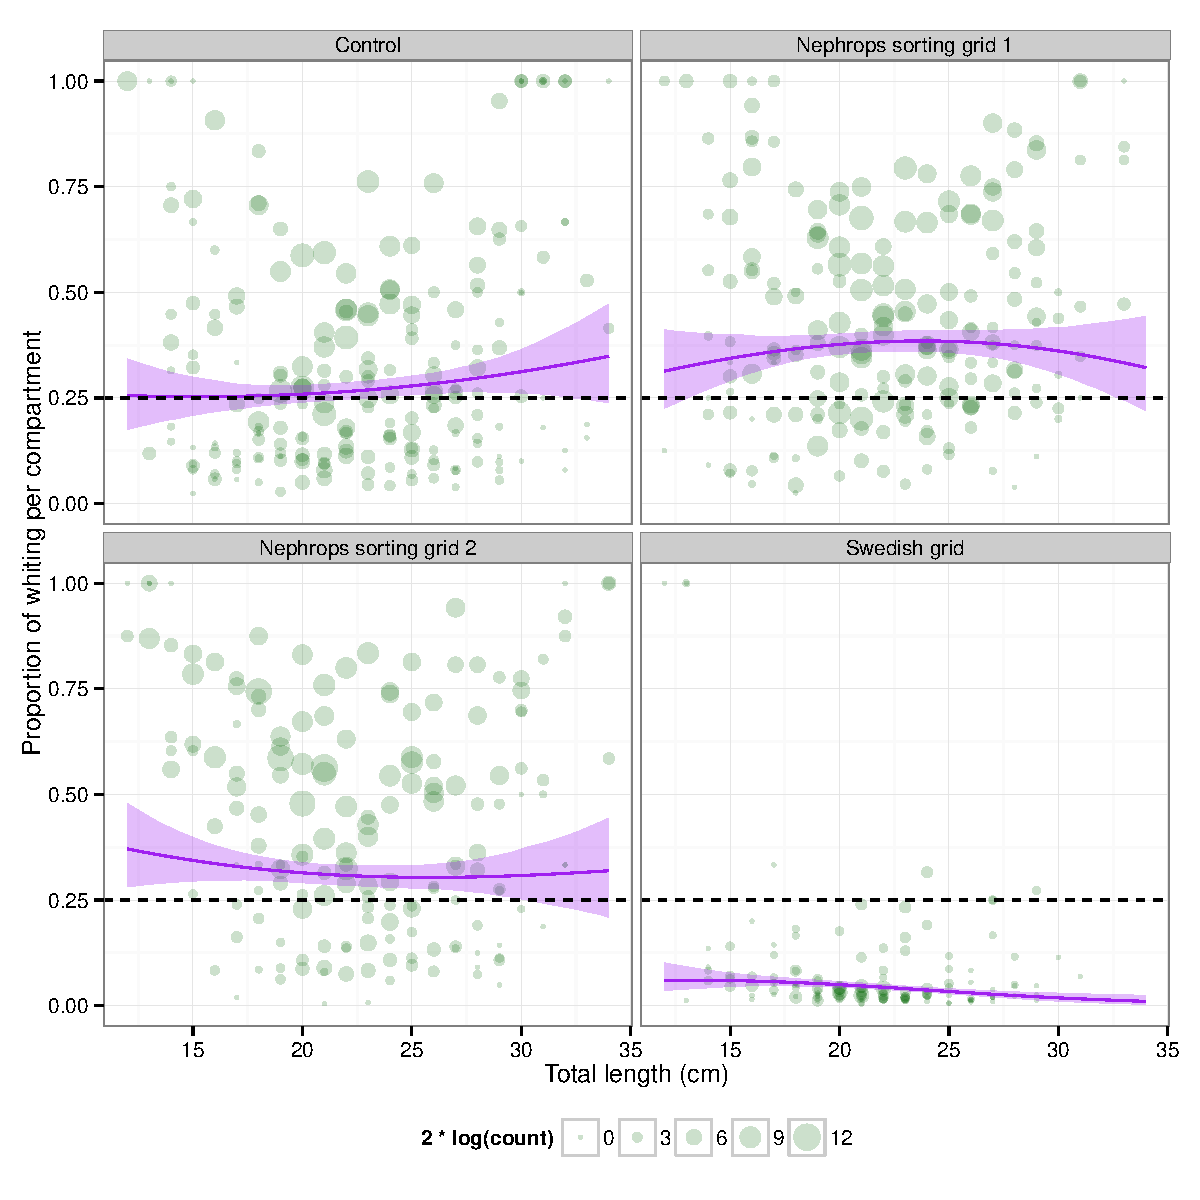
\includegraphics[width=\maxwidth]{figure/unnamed-chunk-8-1} \caption[Proportion of Nephrops catch retained per haul with fitted multinomial model (without a weight effect or random effects) and associated re-sampled intervals]{Proportion of Nephrops catch retained per haul with fitted multinomial model (without a weight effect or random effects) and associated re-sampled intervals. Null hypothesis of equal retention is displayed as the dashed line at 0.25.}\label{fig:unnamed-chunk-8}
\end{figure}


\end{knitrout}

\subsection{Including weight as a covariate}
Here we use the ADMB code to fit weight as a compartment-specific variable. Please note we are working on ways to better integrate this into R.

\begin{knitrout}\footnotesize
\definecolor{shadecolor}{rgb}{0.969, 0.969, 0.969}\color{fgcolor}\begin{kframe}
\begin{alltt}
\hlstd{Yobs} \hlkwb{<-} \hlstd{neph.count.mat}
\hlstd{n} \hlkwb{<-} \hlkwd{nrow}\hlstd{(Yobs)}
\hlstd{m} \hlkwb{<-} \hlkwd{ncol}\hlstd{(Yobs)}
\hlstd{X} \hlkwb{<-} \hlkwd{model.matrix}\hlstd{(best.model)}
\hlcom{## here is where the bulk weights enter}
\hlstd{Xcond} \hlkwb{<-} \hlstd{grid.neph.cast[,} \hlkwd{c}\hlstd{(}\hlstr{"CTRL_Bulk.weight"}\hlstd{,} \hlstr{"NSG1_Bulk.weight"}\hlstd{,}
                            \hlstr{"NSG2_Bulk.weight"}\hlstd{,} \hlstr{"SG_Bulk.weight"}\hlstd{)]}
\hlcom{## hauls}
\hlstd{gps} \hlkwb{<-} \hlkwd{as.numeric}\hlstd{(grid.neph.cast}\hlopt{$}\hlstd{fHAUL)}
\hlstd{ngp} \hlkwb{<-} \hlkwd{length}\hlstd{(}\hlkwd{unique}\hlstd{(gps))}

\hlcom{## predicted values of weight}
\hlcom{## get median bulk weight per net}

\hlstd{median.weights} \hlkwb{<-} \hlkwd{with}\hlstd{(bulk.weight.melt,} \hlkwd{tapply}\hlstd{(value, COMPARTMENT, median))}
\hlstd{median.weights}
\end{alltt}
\begin{verbatim}
##   CTRL   NSG1   NSG2     SG 
## 418.65 346.85 391.00 184.35
\end{verbatim}
\begin{alltt}
\hlcom{## construct the "conditional" prediction matrix}
\hlstd{npred} \hlkwb{<-} \hlkwd{nrow}\hlstd{(Xpred)}
\hlstd{Xcondpred} \hlkwb{<-} \hlkwd{matrix}\hlstd{(median.weights,} \hlkwc{nrow} \hlstd{=} \hlnum{1}\hlstd{)[}\hlkwd{rep}\hlstd{(}\hlnum{1}\hlstd{, npred), ]}

\hlcom{## Output the data to ADMB}
\hlcom{## write the data out}
\hlstd{datfile} \hlkwb{<-} \hlstr{"../admbre/multinomialme.dat"}
\hlkwd{cat}\hlstd{(}\hlstr{"# number of observations n \textbackslash{}n"}\hlstd{, n,} \hlstr{"\textbackslash{}n"}\hlstd{,} \hlkwc{file} \hlstd{= datfile)}
\hlkwd{cat}\hlstd{(}\hlstr{"# number of categories m \textbackslash{}n"}\hlstd{, m,} \hlstr{"\textbackslash{}n"}\hlstd{,} \hlkwc{file} \hlstd{= datfile,} \hlkwc{append} \hlstd{=} \hlnum{TRUE}\hlstd{)}
\hlkwd{cat}\hlstd{(}\hlstr{"# dimension of parameter vector p \textbackslash{}n"}\hlstd{,} \hlkwd{ncol}\hlstd{(X),} \hlstr{"\textbackslash{}n"}\hlstd{,}
    \hlkwc{file} \hlstd{= datfile,} \hlkwc{append} \hlstd{=} \hlnum{TRUE}\hlstd{)}
\hlkwd{cat}\hlstd{(}\hlstr{"# dimension of conditional variables q \textbackslash{}n"}\hlstd{,} \hlkwd{ncol}\hlstd{(Xcond),} \hlstr{"\textbackslash{}n"}\hlstd{,}
    \hlkwc{file} \hlstd{= datfile,} \hlkwc{append} \hlstd{=} \hlnum{TRUE}\hlstd{)}
\hlkwd{cat}\hlstd{(}\hlstr{"# number of groups ngp \textbackslash{}n"}\hlstd{, ngp,} \hlstr{"\textbackslash{}n"}\hlstd{,} \hlkwc{file} \hlstd{= datfile,} \hlkwc{append} \hlstd{=} \hlnum{TRUE}\hlstd{)}
\hlkwd{cat}\hlstd{(}\hlstr{"# response counts Y \textbackslash{}n"}\hlstd{,} \hlkwc{file} \hlstd{= datfile,} \hlkwc{append} \hlstd{=} \hlnum{TRUE}\hlstd{)}
\hlkwd{write.table}\hlstd{(Yobs,} \hlkwc{file} \hlstd{= datfile,} \hlkwc{append} \hlstd{=} \hlnum{TRUE}\hlstd{,}
            \hlkwc{col.names} \hlstd{=} \hlnum{FALSE}\hlstd{,} \hlkwc{row.names} \hlstd{=} \hlnum{FALSE}\hlstd{)}
\hlkwd{cat}\hlstd{(}\hlstr{"# model/design matrix X \textbackslash{}n"}\hlstd{,} \hlkwc{file} \hlstd{= datfile,} \hlkwc{append} \hlstd{=} \hlnum{TRUE}\hlstd{)}
\hlkwd{write.table}\hlstd{(X,} \hlkwc{file} \hlstd{= datfile,} \hlkwc{append} \hlstd{=} \hlnum{TRUE}\hlstd{,}
            \hlkwc{col.names} \hlstd{=} \hlnum{FALSE}\hlstd{,} \hlkwc{row.names} \hlstd{=} \hlnum{FALSE}\hlstd{)}
\hlkwd{cat}\hlstd{(}\hlstr{"# conditional matrix Xcond \textbackslash{}n"}\hlstd{,} \hlkwc{file} \hlstd{= datfile,} \hlkwc{append} \hlstd{=} \hlnum{TRUE}\hlstd{)}
\hlkwd{write.table}\hlstd{(Xcond,} \hlkwc{file} \hlstd{= datfile,} \hlkwc{append} \hlstd{=} \hlnum{TRUE}\hlstd{,}
            \hlkwc{col.names} \hlstd{=} \hlnum{FALSE}\hlstd{,} \hlkwc{row.names} \hlstd{=} \hlnum{FALSE}\hlstd{)}
\hlkwd{cat}\hlstd{(}\hlstr{"# groups \textbackslash{}n"}\hlstd{, gps,} \hlstr{"\textbackslash{}n"}\hlstd{,} \hlkwc{file} \hlstd{= datfile,} \hlkwc{append} \hlstd{=} \hlnum{TRUE}\hlstd{)}
\hlkwd{cat}\hlstd{(}\hlstr{"# Offset (log(q[i]/q[1])) \textbackslash{}n"}\hlstd{,} \hlkwc{file} \hlstd{= datfile,} \hlkwc{append} \hlstd{=} \hlnum{TRUE}\hlstd{)}
\hlkwd{write.table}\hlstd{(offset.mat,} \hlkwc{file} \hlstd{= datfile,} \hlkwc{append} \hlstd{=} \hlnum{TRUE}\hlstd{,}
            \hlkwc{col.names} \hlstd{=} \hlnum{FALSE}\hlstd{,} \hlkwc{row.names} \hlstd{=} \hlnum{FALSE}\hlstd{)}

\hlcom{## predictions}
\hlkwd{cat}\hlstd{(}\hlstr{"# number of prediction rows npred \textbackslash{}n"}\hlstd{, npred,} \hlstr{"\textbackslash{}n"}\hlstd{,}
    \hlkwc{file} \hlstd{= datfile,} \hlkwc{append} \hlstd{=} \hlnum{TRUE}\hlstd{)}
\hlkwd{cat}\hlstd{(}\hlstr{"# prediction matrix Xpred \textbackslash{}n"}\hlstd{,} \hlkwc{file} \hlstd{= datfile,} \hlkwc{append} \hlstd{=} \hlnum{TRUE}\hlstd{)}
\hlkwd{write.table}\hlstd{(Xpred,} \hlkwc{file} \hlstd{= datfile,} \hlkwc{append} \hlstd{=} \hlnum{TRUE}\hlstd{,}
            \hlkwc{col.names} \hlstd{=} \hlnum{FALSE}\hlstd{,} \hlkwc{row.names} \hlstd{=} \hlnum{FALSE}\hlstd{)}
\hlkwd{cat}\hlstd{(}\hlstr{"# conditional prediction matrix Xcondpred \textbackslash{}n"}\hlstd{,}
    \hlkwc{file} \hlstd{= datfile,} \hlkwc{append} \hlstd{=} \hlnum{TRUE}\hlstd{)}
\hlkwd{write.table}\hlstd{(Xcondpred,} \hlkwc{file} \hlstd{= datfile,} \hlkwc{append} \hlstd{=} \hlnum{TRUE}\hlstd{,}
            \hlkwc{col.names} \hlstd{=} \hlnum{FALSE}\hlstd{,} \hlkwc{row.names} \hlstd{=} \hlnum{FALSE}\hlstd{)}

\hlcom{## starting values pinfile}
\hlstd{beta0.start} \hlkwb{<-} \hlkwd{matrix}\hlstd{(}\hlnum{0}\hlstd{,} \hlkwc{nrow} \hlstd{=} \hlkwd{ncol}\hlstd{(X),} \hlkwc{ncol} \hlstd{=} \hlkwd{ncol}\hlstd{(Yobs)} \hlopt{-} \hlnum{1}\hlstd{)}
\hlstd{u0.start} \hlkwb{<-} \hlkwd{matrix}\hlstd{(}\hlnum{0}\hlstd{,} \hlkwc{nrow} \hlstd{= ngp,} \hlkwc{ncol} \hlstd{= m} \hlopt{-} \hlnum{1}\hlstd{)}
\hlstd{nchol} \hlkwb{<-} \hlstd{(m}\hlopt{-}\hlnum{1}\hlstd{)}\hlopt{*}\hlstd{(m)}\hlopt{/}\hlnum{2}
\hlstd{L.start} \hlkwb{<-} \hlkwd{diag}\hlstd{(m}\hlopt{-}\hlnum{1}\hlstd{)}
\hlstd{L.start[}\hlkwd{upper.tri}\hlstd{(L.start)]} \hlkwb{<-} \hlnum{NA}
\hlstd{a.start} \hlkwb{<-} \hlkwd{as.numeric}\hlstd{(}\hlkwd{na.omit}\hlstd{(}\hlkwd{c}\hlstd{(}\hlkwd{t}\hlstd{(L.start))))}
\hlcom{##a.start <- rep(0.1, 3)}

\hlstd{pinfile} \hlkwb{<-} \hlstr{"../admbre/multinomialme.pin"}
\hlkwd{cat}\hlstd{(}\hlstr{"# beta0 \textbackslash{}n"}\hlstd{,} \hlkwc{file} \hlstd{= pinfile)}
\hlkwd{write.table}\hlstd{(beta0.start,} \hlkwc{file} \hlstd{= pinfile,} \hlkwc{append} \hlstd{=} \hlnum{TRUE}\hlstd{,}
            \hlkwc{col.names} \hlstd{=} \hlnum{FALSE}\hlstd{,} \hlkwc{row.names} \hlstd{=} \hlnum{FALSE}\hlstd{)}
\hlkwd{cat}\hlstd{(}\hlstr{"# betacond \textbackslash{}n"}\hlstd{,} \hlnum{0}\hlstd{,} \hlstr{"\textbackslash{}n"}\hlstd{,} \hlkwc{file} \hlstd{= pinfile,} \hlkwc{append} \hlstd{=} \hlnum{TRUE}\hlstd{)}
\hlcom{##set.seed(10)}
\hlkwd{cat}\hlstd{(}\hlstr{"# a \textbackslash{}n"}\hlstd{, a.start,} \hlstr{"\textbackslash{}n"}\hlstd{,} \hlkwc{file} \hlstd{= pinfile,} \hlkwc{append} \hlstd{=} \hlnum{TRUE}\hlstd{)}
\hlcom{##cat("# a \textbackslash{}n", rep(0.1, m-1), "\textbackslash{}n", file = pinfile, append = TRUE)}
\hlkwd{cat}\hlstd{(}\hlstr{"# u0 \textbackslash{}n"}\hlstd{,} \hlkwc{file} \hlstd{= pinfile,} \hlkwc{append} \hlstd{=} \hlnum{TRUE}\hlstd{)}
\hlkwd{write.table}\hlstd{(u0.start,} \hlkwc{file} \hlstd{= pinfile,} \hlkwc{append} \hlstd{=} \hlnum{TRUE}\hlstd{,}
            \hlkwc{col.names} \hlstd{=} \hlnum{FALSE}\hlstd{,} \hlkwc{row.names} \hlstd{=} \hlnum{FALSE}\hlstd{)}

\hlcom{## RUN THE MODEL IN ADMB}
\end{alltt}
\end{kframe}
\end{knitrout}

Plot the model fits

\begin{knitrout}\footnotesize
\definecolor{shadecolor}{rgb}{0.969, 0.969, 0.969}\color{fgcolor}\begin{kframe}
\begin{alltt}
\hlstd{coef.admb} \hlkwb{<-} \hlkwd{read.table}\hlstd{(}\hlstr{"../admbre/multinomialme.std"}\hlstd{,} \hlkwc{header} \hlstd{=} \hlnum{TRUE}\hlstd{)}

\hlcom{##}
\hlstd{p0} \hlkwb{<-} \hlkwd{dim}\hlstd{(X)[}\hlnum{2}\hlstd{]}
\hlstd{beta.hat} \hlkwb{<-} \hlkwd{cbind}\hlstd{(}\hlnum{0}\hlstd{,} \hlkwd{matrix}\hlstd{(}\hlkwd{subset}\hlstd{(coef.admb, name} \hlopt{==} \hlstr{"beta0"}\hlstd{)}\hlopt{$}\hlstd{value,}
                            \hlkwc{nrow} \hlstd{= p0,} \hlkwc{byrow} \hlstd{=} \hlnum{TRUE}\hlstd{))}

\hlstd{betacond.hat} \hlkwb{<-} \hlkwd{subset}\hlstd{(coef.admb, name} \hlopt{==} \hlstr{"betacond"}\hlstd{)}\hlopt{$}\hlstd{value}

\hlcom{## predictions from admb}
\hlstd{eta.hat.admb} \hlkwb{<-} \hlkwd{matrix}\hlstd{(}\hlkwd{subset}\hlstd{(coef.admb, name} \hlopt{==} \hlstr{"etapred"}\hlstd{)}\hlopt{$}\hlstd{value,}
                       \hlkwc{ncol} \hlstd{=} \hlnum{4}\hlstd{,} \hlkwc{byrow} \hlstd{=} \hlnum{TRUE}\hlstd{)}
\hlstd{P.hat.admb} \hlkwb{<-} \hlkwd{exp}\hlstd{(eta.hat.admb)} \hlopt{/} \hlkwd{rowSums}\hlstd{(}\hlkwd{exp}\hlstd{(eta.hat.admb))}
\hlstd{eta.se.admb} \hlkwb{<-} \hlkwd{matrix}\hlstd{(}\hlkwd{subset}\hlstd{(coef.admb, name} \hlopt{==} \hlstr{"etapred"}\hlstd{)}\hlopt{$}\hlstd{std.dev,}
                      \hlkwc{ncol} \hlstd{=} \hlnum{4}\hlstd{,} \hlkwc{byrow} \hlstd{=} \hlnum{TRUE}\hlstd{)}

\hlstd{eta.lwr.admb} \hlkwb{<-} \hlstd{eta.hat.admb} \hlopt{+} \hlkwd{qnorm}\hlstd{(}\hlnum{0.025}\hlstd{)} \hlopt{*} \hlstd{eta.se.admb}
\hlstd{eta.upr.admb} \hlkwb{<-} \hlstd{eta.hat.admb} \hlopt{+} \hlkwd{qnorm}\hlstd{(}\hlnum{0.975}\hlstd{)} \hlopt{*} \hlstd{eta.se.admb}

\hlstd{P.admb.lwr} \hlkwb{<-} \hlkwd{exp}\hlstd{(eta.lwr.admb)} \hlopt{/} \hlkwd{rowSums}\hlstd{(}\hlkwd{exp}\hlstd{(eta.lwr.admb))}
\hlstd{P.admb.upr} \hlkwb{<-} \hlkwd{exp}\hlstd{(eta.upr.admb)} \hlopt{/} \hlkwd{rowSums}\hlstd{(}\hlkwd{exp}\hlstd{(eta.upr.admb))}

\hlstd{plot.pred.df.admb} \hlkwb{<-} \hlkwd{data.frame}\hlstd{(}
                       \hlkwc{COMPARTMENT} \hlstd{=} \hlkwd{rep}\hlstd{(}\hlkwd{c}\hlstd{(}\hlstr{"Control"}\hlstd{,} \hlstr{"Nephrops sorting grid 1"}\hlstd{,}
                           \hlstr{"Nephrops sorting grid 2"}\hlstd{,} \hlstr{"Swedish grid"}\hlstd{),}
                         \hlkwc{each} \hlstd{=} \hlkwd{nrow}\hlstd{(P.hat.admb)),}
                       \hlkwc{Carapace.length} \hlstd{=} \hlkwd{rep}\hlstd{(pred.length,} \hlkwc{times} \hlstd{=} \hlnum{4}\hlstd{),}
                       \hlkwc{proportion} \hlstd{=} \hlkwd{c}\hlstd{(P.hat.admb),}
                       \hlkwc{lwr} \hlstd{=} \hlkwd{c}\hlstd{(P.admb.lwr),}
                       \hlkwc{upr} \hlstd{=} \hlkwd{c}\hlstd{(P.admb.upr))}

\hlstd{p} \hlopt{+} \hlkwd{geom_ribbon}\hlstd{(}\hlkwc{data} \hlstd{= plot.pred.df.admb,} \hlkwd{aes}\hlstd{(}\hlkwc{ymin} \hlstd{= lwr,} \hlkwc{ymax} \hlstd{= upr),}
                \hlkwc{alpha} \hlstd{=} \hlnum{0.3}\hlstd{,} \hlkwc{fill} \hlstd{=} \hlstr{"blue"}\hlstd{)} \hlopt{+}
  \hlkwd{geom_line}\hlstd{(}\hlkwc{data} \hlstd{= plot.pred.df.admb,} \hlkwd{aes}\hlstd{(}\hlkwc{x} \hlstd{= Carapace.length,} \hlkwc{y} \hlstd{= proportion),}
            \hlkwc{col} \hlstd{=} \hlstr{"navy"}\hlstd{,} \hlkwc{size} \hlstd{=} \hlnum{0.5}\hlstd{)} \hlopt{+}
  \hlkwd{geom_hline}\hlstd{(}\hlkwd{aes}\hlstd{(}\hlkwc{yintercept} \hlstd{=} \hlnum{0.25}\hlstd{),} \hlkwc{linetype} \hlstd{=} \hlstr{"dashed"}\hlstd{)}
\end{alltt}
\end{kframe}\begin{figure}
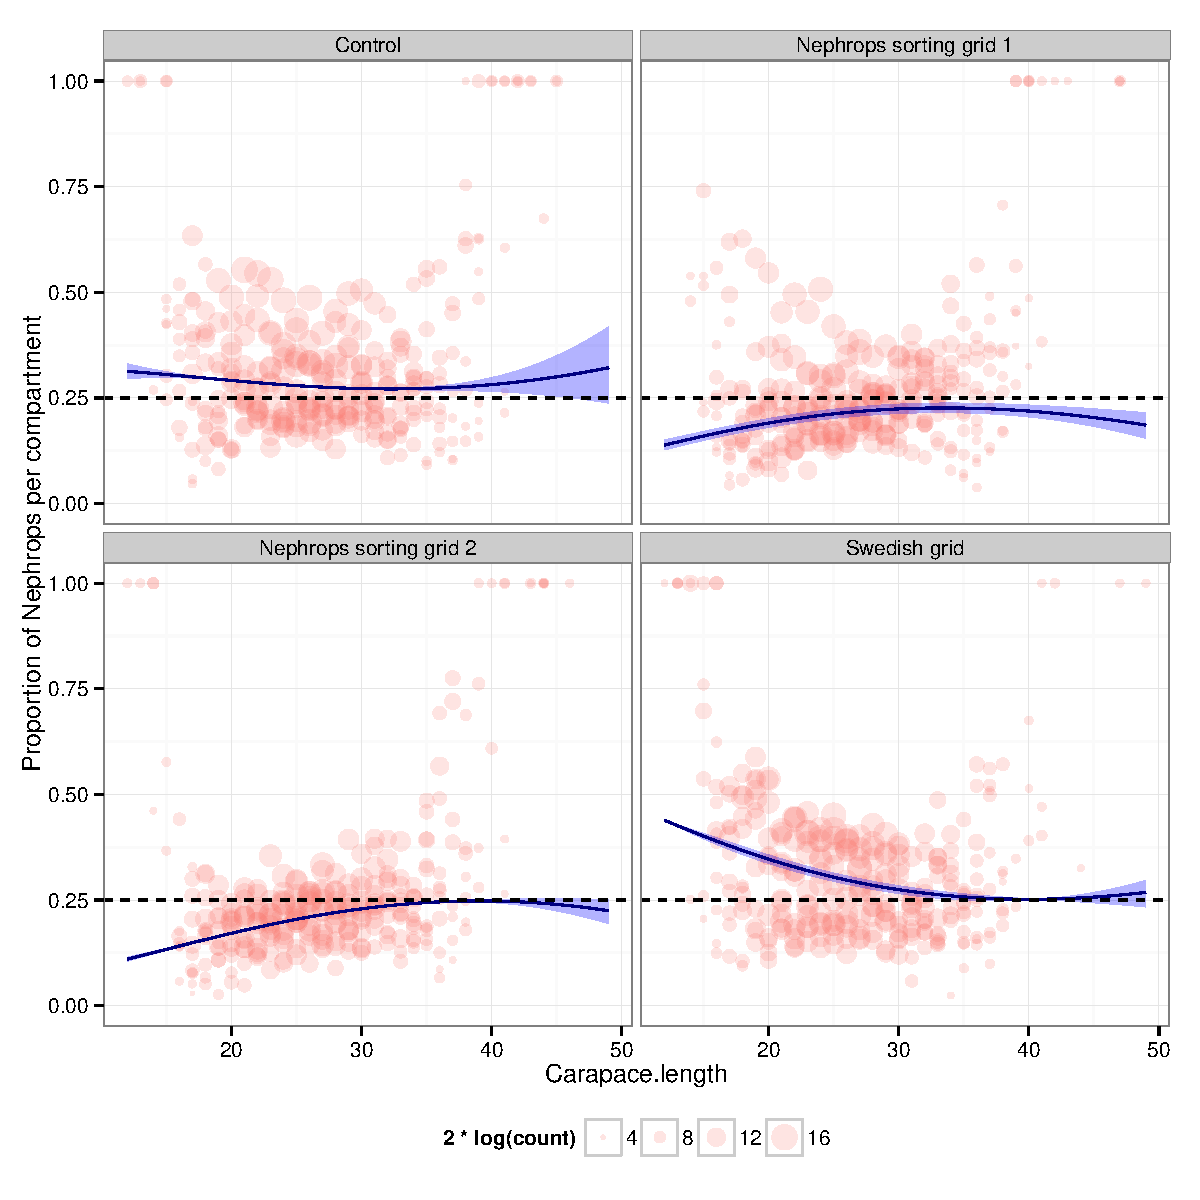
\includegraphics[width=\maxwidth]{figure/unnamed-chunk-10-1} \caption[Proportion of Nephrops catch retained per haul with fitted ADMB multinomial model (with bulk weights set to the mean bulk per compartment)]{Proportion of Nephrops catch retained per haul with fitted ADMB multinomial model (with bulk weights set to the mean bulk per compartment). No random effects were estimated here due to convergence issues which will be investigated.}\label{fig:unnamed-chunk-10}
\end{figure}


\end{knitrout}

Take a look at the random effects
\begin{knitrout}\footnotesize
\definecolor{shadecolor}{rgb}{0.969, 0.969, 0.969}\color{fgcolor}\begin{kframe}
\begin{alltt}
\hlstd{uhat} \hlkwb{<-} \hlkwd{matrix}\hlstd{(}\hlkwd{subset}\hlstd{(coef.admb, name} \hlopt{==} \hlstr{"u0"}\hlstd{)}\hlopt{$}\hlstd{value,} \hlkwc{ncol} \hlstd{= m}\hlopt{-}\hlnum{1}\hlstd{,} \hlkwc{byrow} \hlstd{=} \hlnum{TRUE}\hlstd{)}

\hlkwd{par}\hlstd{(}\hlkwc{mar} \hlstd{=} \hlkwd{c}\hlstd{(}\hlnum{4}\hlstd{,} \hlnum{4}\hlstd{,} \hlnum{2}\hlstd{,} \hlnum{2}\hlstd{))}
\hlkwd{matplot}\hlstd{(}\hlnum{1}\hlopt{:}\hlnum{12}\hlstd{, uhat,} \hlkwc{pch} \hlstd{=} \hlkwd{c}\hlstd{(}\hlnum{2}\hlstd{,} \hlnum{8}\hlstd{,} \hlnum{19}\hlstd{),} \hlkwc{col} \hlstd{=} \hlnum{1}\hlstd{,} \hlkwc{xlab} \hlstd{=} \hlstr{""}\hlstd{,} \hlkwc{ylab} \hlstd{=} \hlstr{""}\hlstd{,} \hlkwc{xaxt} \hlstd{=} \hlstr{"n"}\hlstd{)}
\hlkwd{axis}\hlstd{(}\hlkwc{side} \hlstd{=} \hlnum{1}\hlstd{,} \hlkwc{at} \hlstd{=} \hlnum{1}\hlopt{:}\hlnum{12}\hlstd{,} \hlkwc{labels} \hlstd{=} \hlkwd{c}\hlstd{(}\hlnum{1}\hlopt{:}\hlnum{3}\hlstd{,} \hlnum{5}\hlopt{:}\hlnum{13}\hlstd{))}
\hlkwd{abline}\hlstd{(}\hlkwc{h} \hlstd{=} \hlnum{0}\hlstd{,} \hlkwc{lty} \hlstd{=} \hlnum{2}\hlstd{)}
\hlkwd{mtext}\hlstd{(}\hlkwc{side} \hlstd{=} \hlnum{1}\hlstd{,} \hlkwc{line} \hlstd{=} \hlnum{2.5}\hlstd{,} \hlkwc{text} \hlstd{=} \hlstr{"Haul number"}\hlstd{)}
\hlkwd{mtext}\hlstd{(}\hlkwc{side} \hlstd{=} \hlnum{2}\hlstd{,} \hlkwc{line} \hlstd{=} \hlnum{2.5}\hlstd{,} \hlkwc{text} \hlstd{=} \hlstr{"Log-odds random effects"}\hlstd{)}
\hlkwd{legend}\hlstd{(}\hlstr{"topright"}\hlstd{,} \hlkwc{legend} \hlstd{=} \hlkwd{c}\hlstd{(}\hlstr{"NSG1/CTRL"}\hlstd{,} \hlstr{"NSG2/CTRL"}\hlstd{,} \hlstr{"SG/CTRL"}\hlstd{),} \hlkwc{pch} \hlstd{=} \hlkwd{c}\hlstd{(}\hlnum{2}\hlstd{,} \hlnum{8}\hlstd{,} \hlnum{19}\hlstd{))}

\hlkwd{plot}\hlstd{(}\hlkwd{as.data.frame}\hlstd{(uhat))} \hlcom{## not as strong correlation int he random effects}

\hlcom{## Correlation of the random effects}
\hlstd{a.hat} \hlkwb{<-} \hlkwd{subset}\hlstd{(coef.admb, name} \hlopt{==} \hlstr{"a"}\hlstd{)}\hlopt{$}\hlstd{value}

\hlstd{ii} \hlkwb{<-} \hlnum{1}

\hlstd{L} \hlkwb{<-} \hlkwd{matrix}\hlstd{(}\hlnum{0}\hlstd{,} \hlnum{3}\hlstd{,} \hlnum{3}\hlstd{)}
\hlkwa{for}\hlstd{(i} \hlkwa{in} \hlnum{1}\hlopt{:}\hlnum{3}\hlstd{)\{}
  \hlkwa{for}\hlstd{(j} \hlkwa{in} \hlnum{1}\hlopt{:}\hlstd{i)\{}
    \hlstd{L[i,j]} \hlkwb{<-} \hlstd{a.hat[ii]}
    \hlstd{ii} \hlkwb{<-} \hlstd{ii} \hlopt{+} \hlnum{1}
  \hlstd{\}}
\hlstd{\}}

\hlstd{sigma.hat} \hlkwb{<-} \hlstd{L} \hlopt \hlkwd{t}\hlstd{(L)}

\hlkwd{cov2cor}\hlstd{(sigma.hat)}
\hlkwd{cor}\hlstd{(}\hlkwd{data.frame}\hlstd{(uhat))}
\end{alltt}
\end{kframe}
\end{knitrout}

\begin{knitrout}\footnotesize
\definecolor{shadecolor}{rgb}{0.969, 0.969, 0.969}\color{fgcolor}\begin{kframe}
\begin{alltt}
\hlcom{## Haul level predictions (nest steps)}
\end{alltt}
\end{kframe}
\end{knitrout}



\bibliography{../../../../misc/epif_bibliography}
\bibliographystyle{../../../../misc/cjfas}
\end{document}

